\section{Ragam Hasil Eksperimental \& Analisis Warm Start}

\begin{frame}{Studi Kasus: Entropi Tinggi \& Barren Plateau}
    \begin{columns}
        \begin{column}{0.4\textwidth}
            \textbf{Entropi Tinggi (2021-12-09):}
            \begin{itemize}
                \item Distribusi probabilitas menyebar luas.
            \end{itemize}
            \begin{figure}
                \centering
                
\includegraphics[width=0.7\textwidth]{Laporan/2021-12-09_window.png}
            \end{figure}
        \end{column}
        \begin{column}{0.6\textwidth}
            \textbf{Barren Plateau (2022-06-23 \& 2023-07-05):}
            \begin{itemize}
                \item Hilangnya lanskap gradien secara persisten.
            \end{itemize}
            \begin{figure}
                \centering
                
\includegraphics[width=0.45\textwidth]{Laporan/2022-06-23_window.png}
                
\includegraphics[width=0.45\textwidth]{Laporan/2023-07-05_window.png}
                \caption{Contoh Kejadian Barren Plateau.}
            \end{figure}
        \end{column}
    \end{columns}
\end{frame}

\begin{frame}{Analisis Efektivitas Game Theory (GT) Warm Start (1)}
    \textbf{Keunggulan Strategis Inisialisasi Nash:}
    \begin{itemize}
        \item \textbf{Akurasi Inisialisasi:} Parameter Nash memberikan titik awal yang sangat dekat dengan global minimum, secara efektif menghindari fenomena \textit{stagnasi gradien} atau \textit{Barren Plateau} awal.
        \item \textbf{Efisiensi Komputasi:} Memerlukan jumlah iterasi VQE yang jauh lebih sedikit untuk mencapai ambang batas energi target dibandingkan inisialisasi acak.
        \item \textbf{Penyelarasan Strategis:} Menjamin bahwa solusi kuantum tetap berada dalam koridor keseimbangan pasar (Nash Equilibrium) sejak langkah awal optimasi.
    \end{itemize}
    \begin{block}{Kesimpulan Teknis}
        Integrasi Game Theory sebagai mekanisme pengarah menuju solusi yang lebih reliabel secara finansial.
    \end{block}
\end{frame}

\begin{frame}{Analisis Efektivitas Game Theory (GT) Warm Start (2)}
    \begin{columns}
        \begin{column}{0.45\textwidth}
            \textbf{Dampak pada Performa Portofolio:}
            \begin{itemize}
                \item \textbf{Stabilitas Return:} Kurva pertumbuhan menunjukkan volatilitas yang lebih rendah.
                \item \textbf{Mitigasi Drawdown:} Pengurangan risiko penurunan nilai yang tajam saat anomali pasar.
                \item \textbf{Outperformance:} Akumulasi keuntungan akhir secara signifikan melampaui metode standar.
            \end{itemize}
        \end{column}
        \begin{column}{0.55\textwidth}
            \centering
            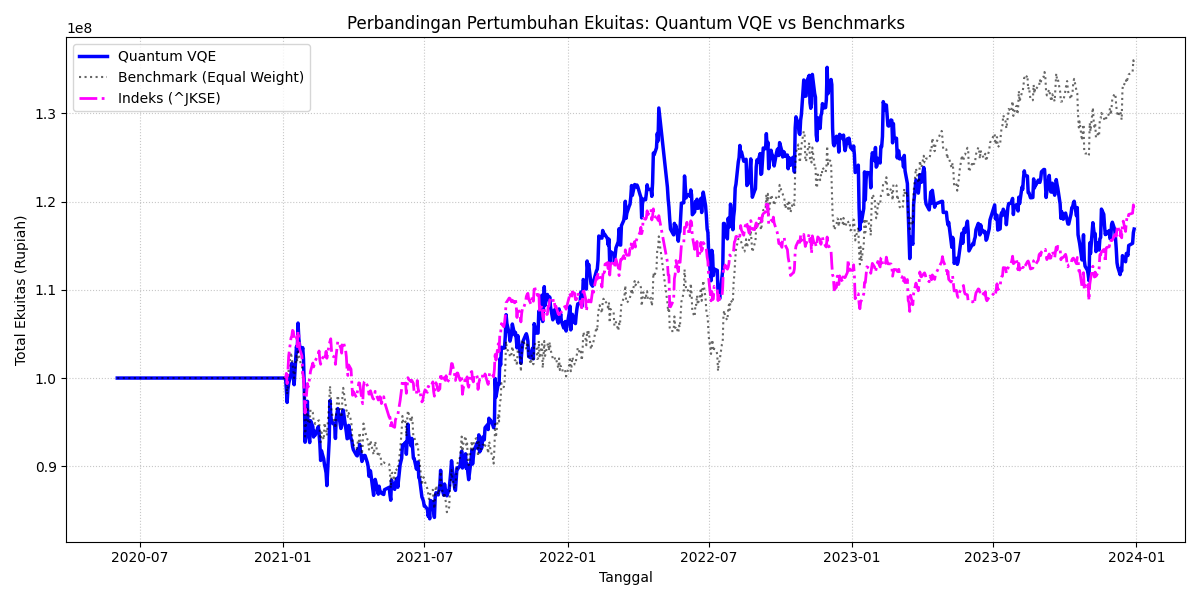
\includegraphics[width=0.6\textwidth]{Laporan/hasil_backtest_vqe_noGT_N4.png}\\
            \small{Tanpa Warm Start (Inisialisasi Acak)}\\
            \vspace{0.2cm}
            
\includegraphics[width=0.6\textwidth]{Laporan/hasil_backtest_vqe_N4.png}\\
            \small{Dengan GT Warm Start (\textbf{Outperform})}
        \end{column}
    \end{columns}
\end{frame}
